\chapter{Accuracy testing}
In order to show the accuracy of the methods and establish a meaningful use of (some of) the library's components, the following method was created.
\begin{figure}[h]
	\centering
	\begin{minipage}[b]{0.5\textwidth}
		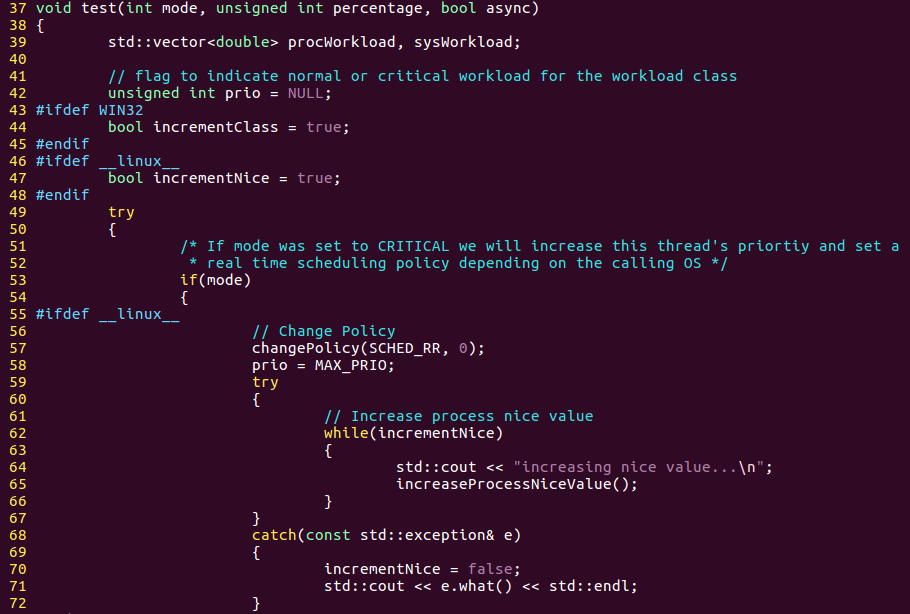
\includegraphics[width=\textwidth]{../figures/testing/testing_method.png}
	\end{minipage}
	\begin{minipage}[b]{0.5\textwidth}
		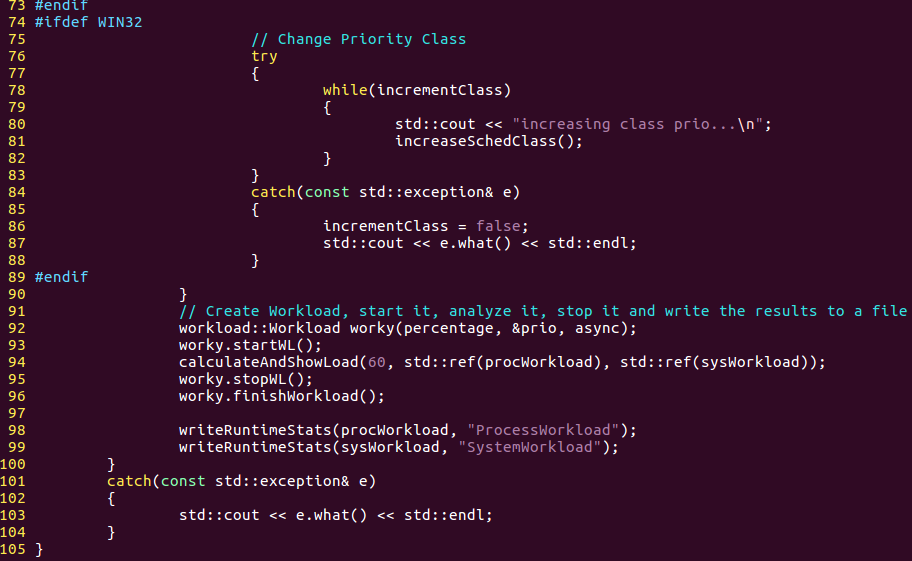
\includegraphics[width=\textwidth]{../figures/testing/testing_method_2.png}
		\caption{Testing method}
	\end{minipage}
\end{figure}
Here we pass the most crucial parameters:
\begin{enumerate}
	\item percentage: in order to specify how big the workload created should be 
	\item async: to verify if the asynchronous mode makes a huge impact on the system
	\item mode: which can be set either to \text{CRITICAL} (define that extends to one) or\\\textit{NORMAL} (define that extends to zero).
\end{enumerate}
The method first defines two lists that will contain the system's and process's workloads. Additionally it sets two flags to true to increase the process's priority (Linux: nice value / Windows: sched class) to maximum and a variable called \textit{prio} to null, which will later be set to \textit{MAX\_PRIO} (defined in \textit{workload.hpp}) to increase the priority of the workload's threads in case the mode was set to critical. The priority's incrementation is called in a \textit{try-catch} block. If this catches an exception we shall set the respective flags to false in order to avoid an endless loop.
Afterwards we create an object of type \textit{Workload} and we pass it the percentage, variable prio's reference and the asny argument. Then we start the workload and call \texttt{calculateAndShowLoad()} in order to see and get the system's statistics. Then we call \texttt{Workload.stopWL()} to stop the loops that create the artificial workload and \texttt{Workload.finishWorkload()} in order to also correctly terminate(join) the started workload threads. At last we use the \texttt{writeRuntimeStats()} function to write the statistics from the lists that we initialised at the begging of the test. This order is necessary for the user to get meaningful results. Small tests in the developing phase of this library showed that computers can't handle well a huge load and IO-operations at the same time. That's why the writing of two or more statistics needs to happen only after the workload was finished. 
 
The method can be called as followed:
\begin{figure}[!htbp]
	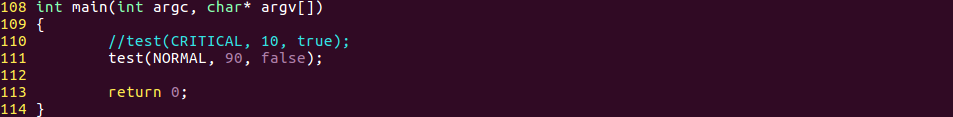
\includegraphics[width=\textwidth]{../figures/testing/main.png}
	\caption{Main testing method}
\end{figure}